% ---------------------------------------------------------------------------
% fragment.tex -- drop-in text for Section 4.4 "The low-mode balanced class for n=4"
% Generated from Analysis/revision/lowmode_n4 (run_all.sh).  All numbers in this
% fragment are in results.json.  Requires \usepackage{booktabs,amsthm,graphicx}.
% ---------------------------------------------------------------------------

\subsection{The low-mode balanced class for $n=4$}
\label{sec:lowmode_n4}

Write $L_n$ for the set of arrangements of $\{1,\dots,n^2\}$ with
$\Cov(X,Z)=\Cov(Y,Z)=\Cov(D_{\mathrm{main}},Z)=\Cov(D_{\mathrm{anti}},Z)=0$,
i.e.\ $E_{\mathrm{low}}=0$.  Each of the four conditions is a \emph{linear} statistic of the
arrangement: with cells indexed by $(i,j)\in\{0,\dots,n-1\}^2$,
$\Cov(X,Z)=0 \iff T_1:=\sum_{i,j} j\,s_{ij} = \tfrac{n-1}{2}\cdot\tfrac{N(N+1)}{2}$,
$\Cov(Y,Z)=0 \iff T_2:=\sum_{i,j} i\,s_{ij}$ equals the same target, and the two diagonal
conditions say that $T_3=\sum_i s_{ii}$ and $T_4=\sum_i s_{i,n-1-i}$ equal $M(n)=n(N+1)/2$.

\begin{proposition}[Exact size of $L_4$]
\label{prop:L4}
$|L_3| = 8$ (the Lo Shu orbit; the class with only $\Cov(X,Z)=\Cov(Y,Z)=0$ has $760$ members), and
\[
  |L_4| \;=\; 14\,639\,440 \;=\; 8\times 1\,829\,930 ,
\]
of which exactly $7040$ are magic squares.  The class is $D_4$-invariant and acts freely
($1\,829\,930$ orbits of size $8$).  The first-moment class
$\{\Cov(X,Z)=\Cov(Y,Z)=0\}$ has $6\,697\,177\,424$ members for $n=4$,
and the class with both diagonals equal to $34$ has $49\,932\,288\,000$ members.
\end{proposition}

\begin{proof}[Computation]
Meet in the middle.  Split the 16 cells into the top two rows $A$ and the bottom two rows $B$.
For each of the $\binom{16}{8}=12\,870$ value sets $V$ and each of the $8!$ bijections $V\to A$,
the partial vector $(T_1,T_2,T_3,T_4)$ restricted to $A$ is packed into a 27-bit integer key; for the
complementary set $V^{c}$ and each bijection $V^{c}\to B$ the vector (target $-$ partial) is
formed, and the number of arrangements is $\sum$ (matching key multiplicities), obtained by
sorting both key lists and merging.  This touches $2\times 12\,870\times 40\,320\approx 1.04\times10^{9}$
partial vectors, against $16!\approx 2.1\times10^{13}$ arrangements for brute force; it runs in
$9$\,s on 16 threads of an Apple M4 Max.  Matching pairs are expanded explicitly to obtain the
row- and column-sum breakdown of \Cref{tab:L4}.  The same program validates on $n=3$
(where brute force is feasible: $8$, $760$, $4224$, $8$ magic, $72$ semi-magic) and, with the
$2n$ line sums in place of $T_1,T_2$, reproduces the $7040$ magic squares and the
$549\,504 = 8\times 68\,688$ semi-magic squares of order 4; the diagonal-only count was also
verified by direct combinatorics, and the probability $|L_4|/16!$ by $2\times10^{9}$ Monte Carlo
samples ($1373$ hits; relative error $2.7\%$).
\end{proof}

\begin{table}[t]
\centering
\caption{Breakdown of $L_4$ by the number of row sums and column sums equal to $M(4)=34$.
Exactly two or three equal row sums are impossible: if $R_i=34+e_i$ then $\sum_i e_i=0$ and
$\sum_i i\,e_i=0$ (this is $T_2$), which cannot hold with exactly one or two nonzero $e_i$;
the same holds for columns.  The table is symmetric under transposition.}
\label{tab:L4}
\begin{tabular}{lrrrr}
\toprule
 & \multicolumn{4}{c}{columns equal to 34} \\
\cmidrule(lr){2-5}
rows equal to 34 & 0 & 1 & 4 & total \\
\midrule
0 & 9\,637\,312 & 2\,172\,824 & 100\,728 & 11\,910\,864 \\
1 & 2\,172\,824 & 429\,312 & 9\,336 & 2\,611\,472 \\
4 & 100\,728 & 9\,336 & \textbf{7\,040} (magic) & 117\,104 \\
\midrule
total & 11\,910\,864 & 2\,611\,472 & 117\,104 & 14\,639\,440 \\
\bottomrule
\end{tabular}
\end{table}

Thus only $7040/14\,639\,440 = 0.048\%$ of the low-mode balanced arrangements are magic;
$110\,064$ members have all row sums equal to 34 but not all column sums (and symmetrically),
and $9\,637\,312$ (66\%) have \emph{no} row or column summing to $34$ at all.  The arrangement
exhibited in the Appendix belongs to the last class.  \Cref{fig:lowmode_gallery} shows one member
from each of six classes.

\paragraph{Why random sampling never found a counterexample.}
$|L_4|/16! = 6.997\times10^{-7}$, about one arrangement in $1.43$ million: $460$ million uniform
samples are expected to contain about $322$ members of $L_4$ (but only $0.15$ magic squares), so the
estimate ``below $10^{-8}$'' given in v4 for this probability was too small by a factor of about $70$,
and the absence of non-magic zeros in the earlier sampling runs cannot be explained by rarity alone.
A Gaussian local-limit estimate explains the order
of magnitude: under a uniform random permutation the vector $(T_1,T_2,T_3,T_4)$ has mean equal to the
target vector and covariance $\Sigma_{mk} = \frac{1}{N-1}\sum_c (a_{m,c}-\bar a_m)(a_{k,c}-\bar a_k)\sum_v (v-\bar v)^2$,
where $a_m$ is the weight vector of $T_m$ (Hoeffding's permutation variance identity).  $T_1,T_2$ are
uncorrelated with each other and with the diagonals; the two diagonals have correlation $-1/(n^2-1)$
for even $n$ and $0$ for odd $n$.  The achievable values of $(T_1,\dots,T_4)$ form the full lattice
$\mathbb{Z}^4$ (checked via a Smith normal form of the single-transposition steps for $n\le 8$), so
\[
  |L_n| \;\approx\; N!\,(2\pi)^{-2}\det(\Sigma)^{-1/2}.
\]
The estimate gives $13.6$ for $n=3$ (true: $8$, ratio $0.59$) and $1.82\times10^{7}$ for $n=4$ (true:
$14\,639\,440$, ratio $0.80$); for the two-condition classes the ratios are $0.59/0.91$ (first moments)
and $1.10/0.96$ (diagonals), so the Gaussian approximation improves with $n$ as the local limit theorem
predicts.  For larger $n$ we have no exact count; the estimate and a Monte Carlo check are
\begin{align*}
  |L_5| &\approx 6.7\times10^{17}\ \text{(Gaussian)}, & &5.1\times10^{17}\ \text{(Monte Carlo, $10^{10}$ samples, $\pm 6\%$)},\\
  |L_6| &\approx 1.5\times10^{33}\ \text{(Gaussian)}, & &1.2\times10^{33}\ \text{(Monte Carlo, $2\times10^{10}$ samples, $\pm 13\%$)},
\end{align*}
to be read as conjectural orders of magnitude ($25!\approx1.6\times10^{25}$, $36!\approx3.7\times10^{41}$).
In every case the magic squares are a vanishing fraction of $L_n$: the four low-mode conditions
cost a factor of order $\det(\Sigma)^{1/2}\propto n^{13}$ (two first-moment statistics of standard
deviation $\sim n^{4}/12$ and two diagonal sums of standard deviation $\sim n^{5/2}$), while a magic
square requires $2n$ independent line conditions, each costing a further factor of order $n^{5/2}$.

\begin{figure}[t]
\centering
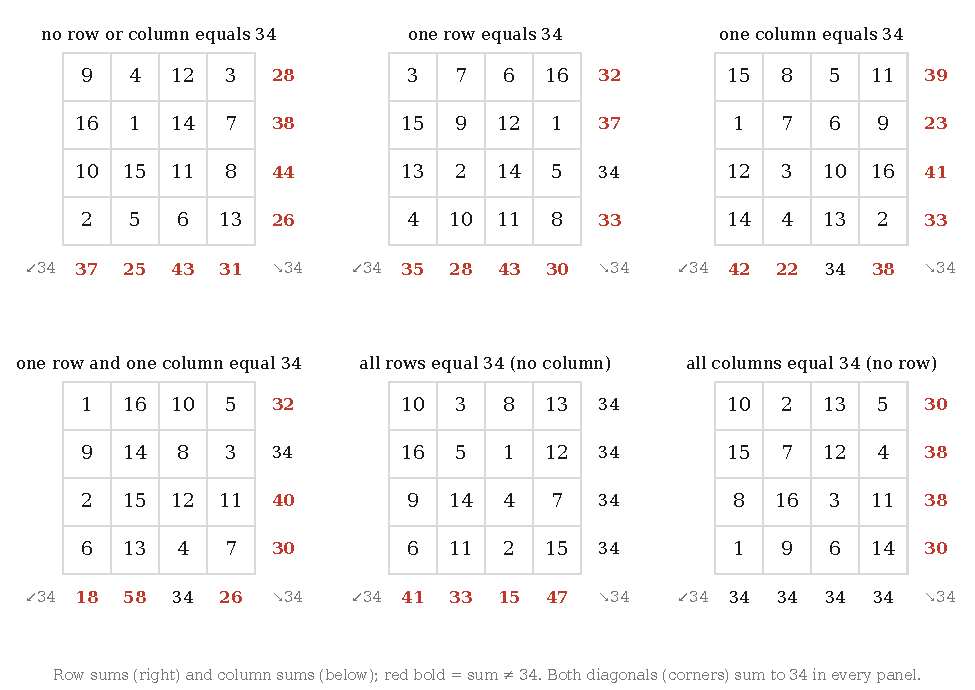
\includegraphics[width=\textwidth]{fig_lowmode_gallery.pdf}
\caption{Six non-magic members of $L_4$, one from each class of \Cref{tab:L4} other than the
magic squares and the two mixed classes $(4,1)$, $(1,4)$.  Row sums are printed to the right of each
square and column sums below it; sums different from $34$ are in red.  Both diagonals (corner
annotations) sum to $34$ in every panel, and in every panel $\sum_j j\,C_j=\sum_i i\,R_i = 204$,
so $E_{\mathrm{low}}=0$ although $E_{\mathrm{full}}>0$.  Top left: the counterexample of the Appendix.}
\label{fig:lowmode_gallery}
\end{figure}

% Optional second figure:
% \begin{figure}[t]\centering
% 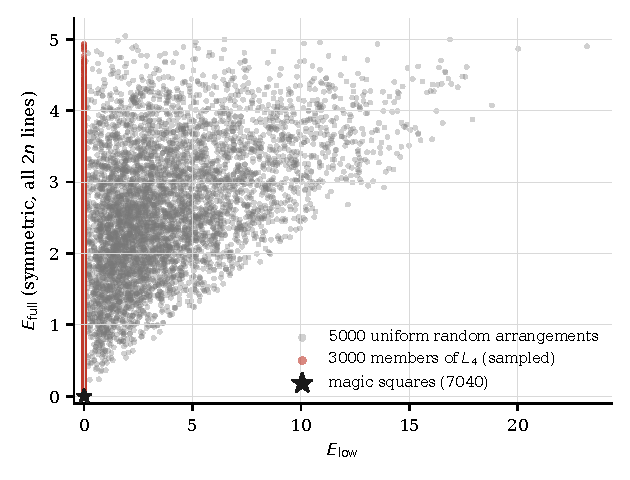
\includegraphics[width=0.6\textwidth]{fig_lowmode_vs_full_n4.pdf}
% \caption{$E_{\mathrm{low}}$ against the symmetric $E_{\mathrm{full}}$ for $5000$ uniform random
% $4\times4$ arrangements (grey) and $3000$ members of $L_4$ (red, all at $E_{\mathrm{low}}=0$ with
% $E_{\mathrm{full}}$ between $1/64$ and $5.3$); the magic squares sit at the origin.}
% \label{fig:lowmode_vs_full}\end{figure}
